\documentclass[a4paper, 12pt]{article}

\usepackage[utf8]{inputenc}
\usepackage[margin=2.5cm]{geometry}
\usepackage{hyperref}
\usepackage{graphicx}

\renewcommand*\contentsname{Table des matières}
\renewcommand{\familydefault}{\sfdefault}

\title{
	\hrulefill
	\\
	Manuel d'installation
	\\
	\textbf{Guardians Studio} \\
	\hrulefill

}
\author{Alexandre Privat - Erwann Lesech - Guillaume Jolivalt - Raphaël Heng}
\date{EPITA Lyon $|$ Promo 2026}

\begin{document}
	\maketitle
	\begin{figure}[ht]
		\centering
		
\includegraphics[width=10cm, height=10cm]{images/logo.png}
	\end{figure}
	\clearpage
	\tableofcontents
	
	\clearpage
	
	\section{Version Portable}
	\subsection{Pour télécharger le launcher}
	Rendez vous sur la page téléchargements de notre site :
	\url{https://guardiansstudio.000webhostapp.com/download.php}.
	Puis scrollez vers le bas jusqu'à voir le bouton "Télécharger le jeu (Launcher Portable)" et cliquez dessus pour lancer le téléchargement.
	
	\begin{figure}[ht]
		\centering
		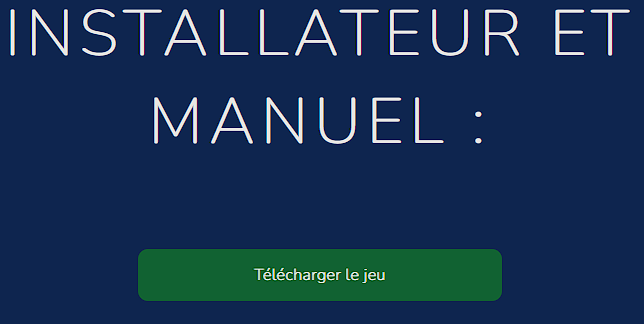
\includegraphics[scale=0.6]{images/download_launcher.png}
		\caption{Boutons de téléchargements du jeu}
	\end{figure}
	
	Le fichier devrait s'appeler \textit{Era\_Of\_Guardians\_TV\_Launcher.zip}.
	
	\subsection{Après avoir téléchargé le launcher}
	Il faut ensuite décompresser le fichier \textit{Era\_Of\_Guardians\_TV\_Launcher.zip}. Vous pouvez utiliser le logiciel open-source \href{https://www.7-zip.fr/}{7-zip} ou utiliser l'outil par défaut de Windows pour le faire. Si vous souhaitez installer 7-zip, vous devez vous rendre sur la page puis télécharger l'exécutable correspondant à l'architecture de votre ordinateur (pour la majorité des personnes, ce sera 64 bits). Ensuite il faudra lancer l'exécutable et vous pourrez extraire avec 7-zip comme ceci :
	
	\begin{figure}[ht]
		\centering
		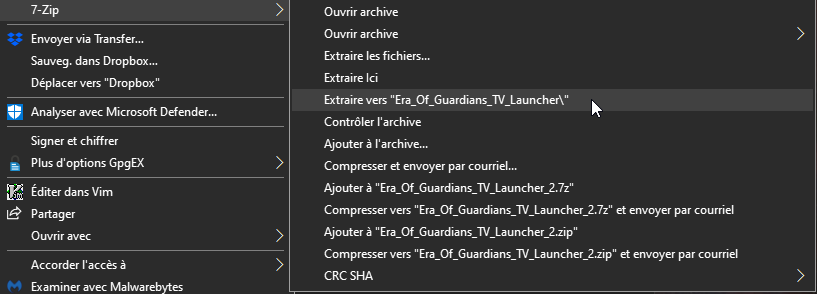
\includegraphics[scale=0.6]{images/7zip_menu.png}
		\caption{Menu contextuel de 7-zip}
	\end{figure}
	
	Vous aurez ensuite un dossier \textit{Era\_Of\_Guardians\_TV\_Launcher}, ouvrez-le et vous trouverez plusieurs 
	fichiers
	
	\begin{figure}[ht]
		\centering
		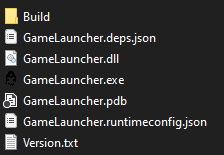
\includegraphics[scale=0.8]{images/fichiers.png}
		\caption{Fichiers du launcher}
	\end{figure}

	Il faut lancer le fichier intitulé \textit{GameLauncher.exe}. L'interface devrait ressembler à ceci :
	\clearpage
	\begin{figure}[ht]
		\centering
		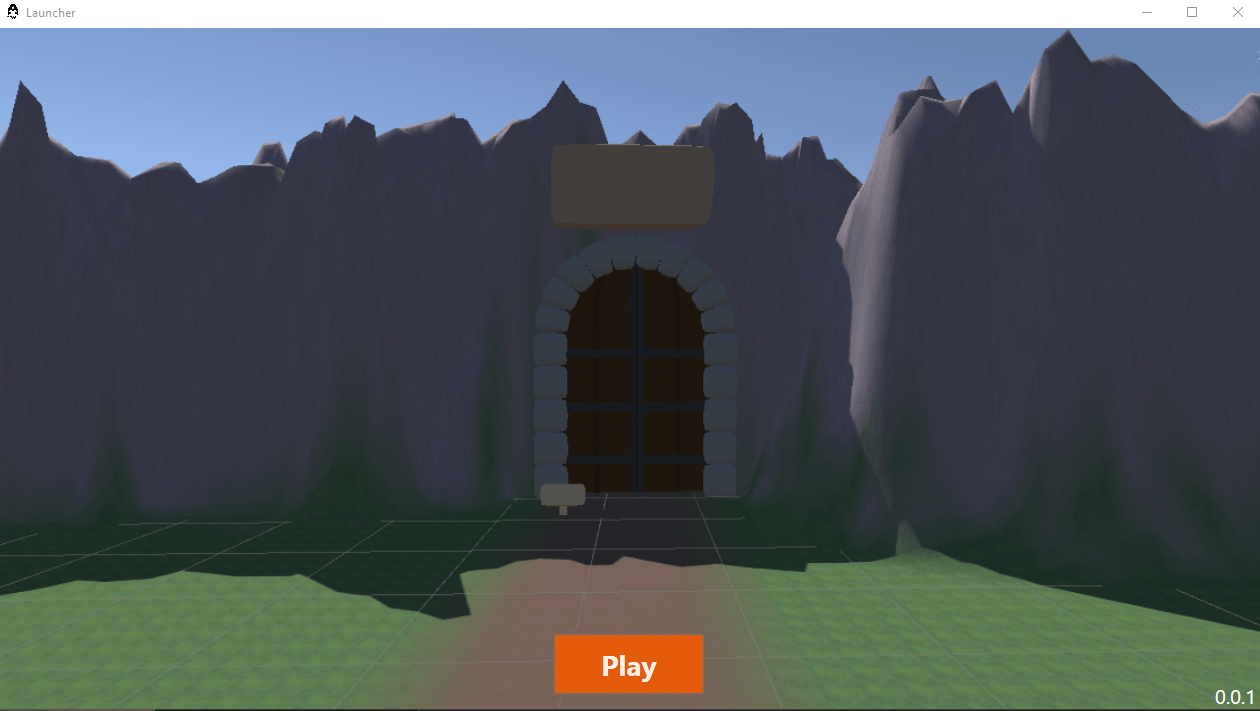
\includegraphics[scale=0.4]{images/launcher.png}
		\caption{Interface du launcher}
	\end{figure}

	Si le bouton n'est pas "Play", il faut attendre que le logiciel vérifie la présence d'éventuelles mises à jour et les télécharge si besoin. Le numéro en bas à droite correspond à la version du jeu. Dès que "Play" apparaît, vous pouvez cliquer dessus pour lancer le jeu.
	
	
	
	\subsection{Pour désinstaller le Launcher}
	Il suffit de supprimer le dossier contenant les fichiers du jeu et l'archive.
	
	\section{Version Setup}
	\subsection{Pour télécharger le setup}
	Rendez vous sur la page téléchargements de notre site :
	\url{https://guardiansstudio.000webhostapp.com/download.php}.
	Puis scrollez vers le bas jusqu'à voir le bouton "Télécharger le jeu (Setup)" et cliquez dessus pour lancer le téléchargement.
	
	\begin{figure}[ht]
		\centering
		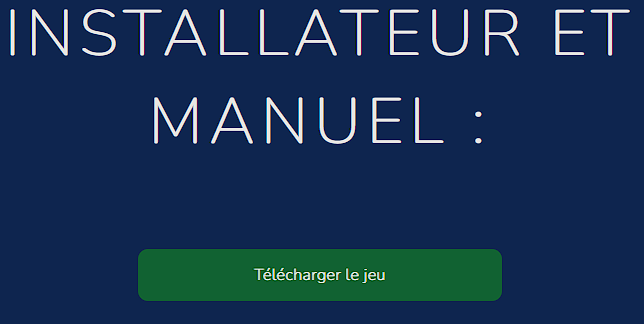
\includegraphics[scale=0.6]{images/download_launcher.png}
		\caption{Boutons de téléchargements du jeu}
	\end{figure}
	
	\subsection{Après avoir téléchargé le setup}
	Il suffit de l'exécuter (le fichier s'appelle Era-Of-Guardians-Setup-version.exe) et de suivre les instructions à l'écran.
	Il est recommandé de laisser le chemin d'installation par défaut et de mettre un raccourci sur le bureau.
	\subsection{Pour désinstaller le setup}
	Un exécutable de désinstallation (unins0000.exe) est fourni, il se trouve dans le dossier dans lequel vous avez installé le jeu (par défaut C:\textbackslash Programmes (x86)\textbackslash Era Of Guardians TV).  
	
	\section{En cas d'erreur après installation}
	Si vous avez une erreur de ce type : 
	\begin{figure}[ht]
		\centering
		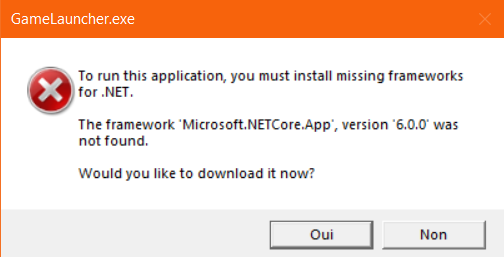
\includegraphics[scale=0.4]{images/erreur.png}
		\caption{Erreur s'il manque le framework .NET}
	\end{figure}
	\\
	Il faut cliquer sur "Oui" et cela va vous amener sur \href{https://dotnet.microsoft.com/en-us/download/dotnet/6.0/runtime?cid=getdotnetcore}{cette page}.
	Pour la  majorité des personnes, le bon lien serait celui-ci : 
	\begin{figure}[h!]
		\centering
		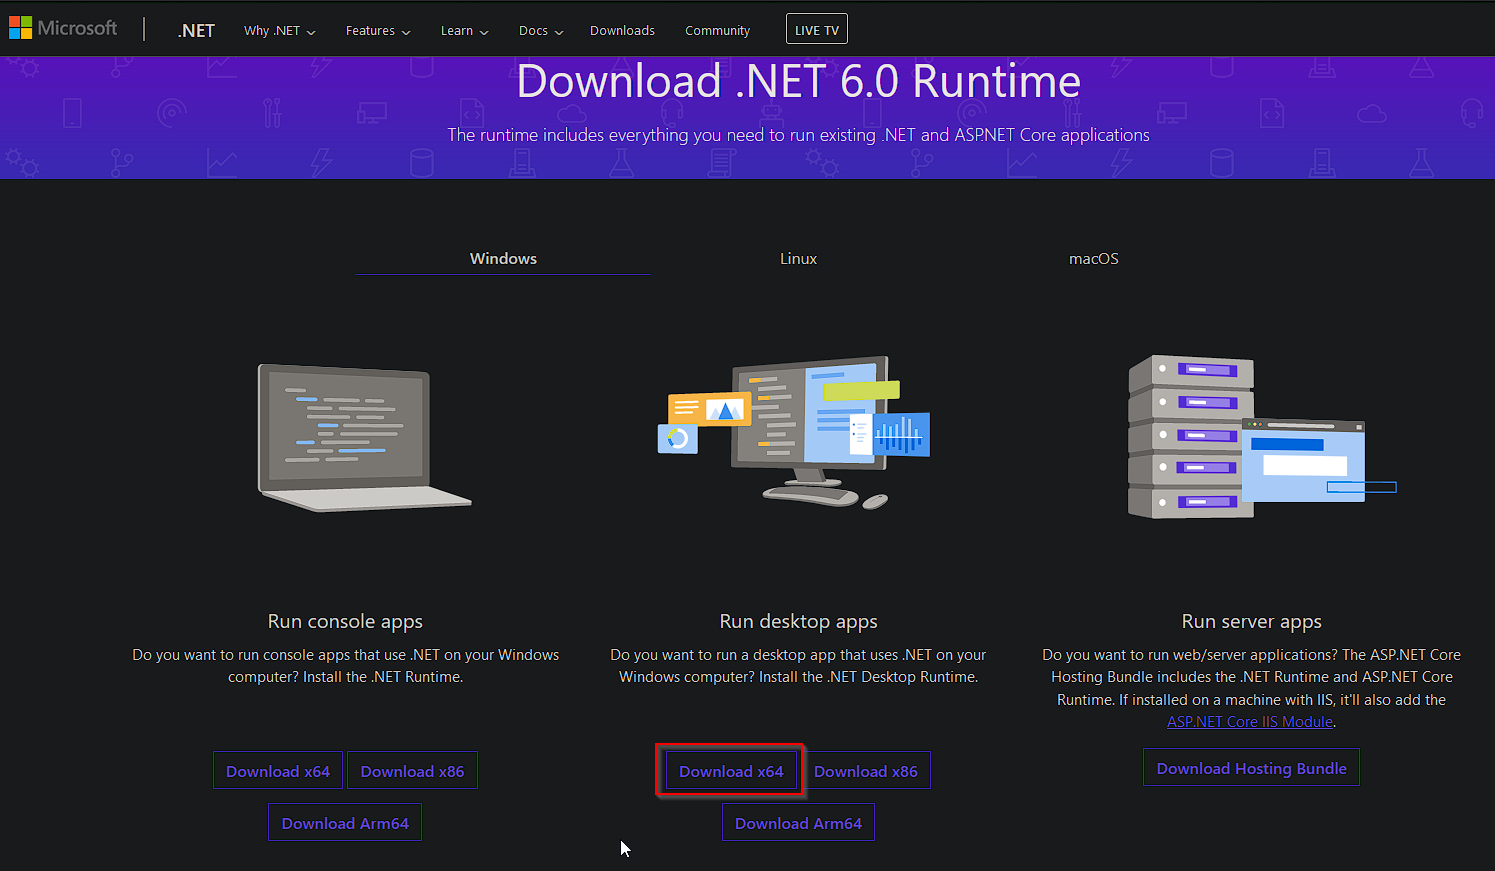
\includegraphics[scale=0.35]{images/dotnet.png}
		\caption{Téléchargement .NET}
	\end{figure}	
	
\end{document}